% ICARC paper
% Build in VS Code (LaTeX Workshop): open this file and press Ctrl+Alt+B, or save it.
% View the PDF: Ctrl+Alt+V.  Command line: latexmk -pdf main.tex
\documentclass[conference,a4paper]{IEEEtran}
\IEEEoverridecommandlockouts

% Page layout of the IEEE A4 conference template (IEE conference template/conference-template-a4.docx):
% A4, top 0.75 in, bottom 1 in, left/right 16 mm, 0.25 in between the two columns.
\usepackage[a4paper, top=19.05mm, bottom=25.4mm, left=16mm, right=16mm, columnsep=6.35mm]{geometry}

\usepackage{cite}
\usepackage{amsmath,amssymb,amsfonts}
\usepackage{graphicx}
\usepackage{textcomp}
\usepackage{xcolor}
\usepackage{multirow}
\usepackage{array}
\usepackage{makecell}
\usepackage{url}
\usepackage{xspace}
\usepackage{tikz}
\usetikzlibrary{positioning,arrows.meta,fit,backgrounds,calc}

% Figure, table and keyword settings requested by the supervisor (comment 16)
\usepackage{balance}
\usepackage{caption}
\DeclareCaptionFormat{figureformat}{#1#2. #3}
\captionsetup[figure]{format=figureformat, justification=raggedright, singlelinecheck=false, font=footnotesize, labelsep=none}
\DeclareCaptionFormat{tableformat}{\textsc{#1}#2. \textsc{#3}}
\captionsetup[table]{format=tableformat, labelsep=none, font=footnotesize}  % 8 pt, as the template's table head
\def\BibTeX{{\rm B\kern-.05em{\sc i\kern-.025em b}\kern-.08em
    T\kern-.1667em\lower.7ex\hbox{E}\kern-.125emX}}
\setlength{\parskip}{6pt}
\renewcommand\IEEEkeywordsname{Keywords}

% Tables: all horizontal and vertical borders, as in the template.
\renewcommand{\arraystretch}{1.15}
% Table footnote, 8 pt (template style "table footnote").
\newcommand{\tablenote}[1]{\par\vspace{2pt}{\scriptsize #1}}

% ---------------------------------------------------------------------------
% Draft helpers. Set \draftfalse before submission: every TBD/TODO disappears,
% so the compile log (and a search for "TBD") shows anything still missing.
\newif\ifdraft
\drafttrue
\ifdraft
  \newcommand{\TBD}[1][]{\textcolor{red}{[TBD#1]}\xspace}
  \newcommand{\todo}[1]{\textcolor{blue}{[TODO: #1]}}
\else
  \newcommand{\TBD}[1][]{}
  \newcommand{\todo}[1]{}
\fi
% ---------------------------------------------------------------------------

\begin{document}

\title{Generalized Deep Reinforcement Learning for Traffic Signal Control}

\author{
\IEEEauthorblockN{Lakshitha Konara}
\IEEEauthorblockA{\textit{Department of Computer Science and Engineering} \\
\textit{University of Moratuwa}\\
Moratuwa, Sri Lanka \\
lakshithakonara3@gmail.com}
\and
\IEEEauthorblockN{Dulani Meedeniya}
\IEEEauthorblockA{\textit{Department of Computer Science and Engineering} \\
\textit{University of Moratuwa}\\
Moratuwa, Sri Lanka \\
dulanim@cse.mrt.ac.lk}
}

\maketitle

\begin{abstract}
Deep reinforcement learning (DRL) controllers for adaptive traffic signals are usually trained and tested on the same hour of traffic, which hides whether they generalize to traffic they have not seen. This paper evaluates whether DRL signal controllers generalize to demand levels not encountered during training. Using three real-city scenarios of the RESCO benchmark from Cologne and Ingolstadt in the SUMO simulator, we train DQN, Double DQN, PPO and A2C on seeded variants of the real peak hour with 0.8 to 1.2 times its traffic, select models on separate validation variants, and test them on 0.7 and 1.3 times the traffic and on the original hour, against fixed-time and tuned actuated control over five training seeds. A2C performs best in all three scenarios. On the two single-intersection scenarios its average total waiting time per vehicle is 13.5 s and 10.0 s, against 32.5 s and 24.2 s for fixed-time control, and 25.2 s and 23.2 s at the unseen heavy demand, against 52.3 s and 48.8 s. On the three-intersection scenario every learner occasionally gridlocks the network. A2C does so in 1 of 50 test episodes and averages 25.5 s against 30.9 s for fixed-time control. An ablation shows that removing demand randomization or policy sharing, or adding valid-action masking, leaves typical waiting times unchanged, while failure counts vary as much between seeds as between variants.
\end{abstract}

\vspace{6pt}
\begin{IEEEkeywords}
deep reinforcement learning, generalization, policy sharing, SUMO, traffic signal control
\end{IEEEkeywords}

\section{Introduction}
\label{sec:intro}

Traffic congestion at signalized intersections costs travel time, fuel and safety in cities worldwide. Most intersections still run fixed-time plans, which repeat the same cycle regardless of traffic, or actuated control, which stretches or cuts a green phase when loop detectors report arriving vehicles~\cite{michailidis2025review}. Deep reinforcement learning (DRL) offers a data-driven alternative: an agent at each intersection observes the queues on its approaches and chooses the next green phase, learning a policy that reduces delay~\cite{michailidis2025review,mei2024libsignal}.

Two gaps make it hard to tell how such controllers would perform in practice. First, evaluation rarely separates training and test demand. A scenario typically ships one hour of calibrated traffic, and many studies train and report on that same hour, so a controller can perform well by memorizing one demand pattern~\cite{ault2021resco,kwesiga2026robustness}. Second, algorithm comparisons are rarely controlled: learners are reported with different observations, rewards, yellow times and numbers of seeds, so differences can come from the setup rather than the algorithm~\cite{mei2024libsignal,agarwal2021precipice}.

This work is useful to traffic agencies and researchers who must choose a DRL controller before deploying it: it shows which widely used algorithm keeps its benefit when traffic differs from the training data, how often each one fails, and what the failures look like, and it provides a reusable protocol for such tests. It is also the first stage of a larger study on resource-aware edge--cloud intelligent transportation systems. We compare DQN, Double DQN, PPO and A2C because they represent the two main DRL families used for signal control: value-based off-policy learning (DQN, and Double DQN, which corrects DQN's over-estimation of action values) and on-policy actor-critic learning (A2C, and PPO, which limits the size of each policy update). Independent DQN and PPO learners were also the strongest methods on the RESCO benchmark~\cite{ault2021resco}, and all four have mature, directly comparable implementations~\cite{raffin2021sb3}. As real-city scenarios we use cologne1, ingolstadt1 and cologne3 from RESCO~\cite{ault2021resco}, which provide real road geometry and calibrated peak-hour demand from the TAPASCologne and InTAS traffic models.

The contributions of this study are: (i) a generalization-focused protocol that trains on $0.8$--$1.2\times$ variants of the real peak hour and tests only on unseen $0.7\times$ and $1.3\times$ demand and on the original hour; (ii) a controlled comparison of DQN, Double DQN, PPO and A2C against fixed-time, tuned actuated and random control with identical observations, rewards, yellow times and interaction budgets, and five seeds each; (iii) a failure analysis showing that rare gridlock episodes, rather than average performance, separate the learners; and (iv) an ablation of the two training components, demand randomization and policy sharing, and of valid-action masking, with per-intersection results that locate the failures. The generalization-focused evaluation of DRL signal controllers on demand levels not encountered during training is considered the main novelty.

\section{Related Work}
\label{sec:related}

DRL controllers select signal phases from queue, density and pressure features, using value-based and actor-critic learners at single intersections and across networks~\cite{michailidis2025review}. LibSignal~\cite{mei2024libsignal} compares ten such methods on common datasets in the SUMO~\cite{lopez2018sumo} and CityFlow simulators, and the RESCO benchmark~\cite{ault2021resco} standardized evaluation on real-city SUMO scenarios of Cologne and Ingolstadt, where independent DQN and PPO learners outperformed more specialized coordinated methods. Both compare algorithms on the demand they were trained on. Generalization has been studied for other kinds of change: UniTSA~\cite{wang2024unitsa} uses a junction matrix and traffic-state augmentation so that one policy works across intersections with different layouts, and $\pi$-Light~\cite{gu2024pilight} learns compact programmatic policies that transfer across intersections in different cities. Kwesiga et al.~\cite{kwesiga2026robustness} showed that a controller trained on one origin--destination pattern generalizes only to similar demand, while diverse training patterns improve robustness, and Sim2Signal~\cite{rafi2026sim2signal} benchmarks the simulation-to-reality gap. Compact controllers for limited roadside hardware have also been proposed~\cite{xing2022tinylight,gu2024pilight}.

Table~\ref{tab:related} summarizes these studies. With the exception of the sim-to-real benchmark, they either test generalization with a single proposed method or compare several algorithms without a generalization test. To our knowledge, no prior study compares several DRL algorithm families under one controlled protocol on real-city scenarios, tests every learner on demand levels unseen in training, and isolates the effect of each training component with an ablation; this combination is the novelty of the present work.

\begin{table}[t]
\caption{Comparison with Related Studies}
\label{tab:related}
\centering
\footnotesize
\setlength{\tabcolsep}{3pt}
\begin{tabular}{|l|>{\raggedright\arraybackslash}p{3.0cm}|c|c|}
\hline
\textbf{Study} & \textbf{Approach} & \textbf{\makecell{Gen.\\test\textsuperscript{a}}} & \textbf{\makecell{Alg.\\comp.\textsuperscript{b}}} \\
\hline
RESCO~\cite{ault2021resco}, 2021 & IDQN, IPPO, MPLight, FMA2C & $\times$ & \checkmark \\
\hline
LibSignal~\cite{mei2024libsignal}, 2024 & Open library, ten methods & $\times$ & \checkmark \\
\hline
UniTSA~\cite{wang2024unitsa}, 2024 & Universal RL with state augmentation & \checkmark & $\times$ \\
\hline
$\pi$-Light~\cite{gu2024pilight}, 2024 & Programmatic policy & \checkmark & $\times$ \\
\hline
Kwesiga et al.~\cite{kwesiga2026robustness}, 2026 & RL with ring-barrier phases & \checkmark & $\times$ \\
\hline
Sim2Signal~\cite{rafi2026sim2signal}, 2026 & Sim-to-real benchmark & \checkmark & \checkmark \\
\hline
This work & DQN, DDQN, PPO, A2C & \checkmark & \checkmark \\
\hline
\end{tabular}
\tablenote{\textsuperscript{a}Tested on conditions not seen in training. \textsuperscript{b}Several RL algorithms compared under one protocol. \todo{verify every tick against the full papers}}
\end{table}

\section{Problem Formulation}
\label{sec:problem}

A road network contains a set $\mathcal{I}$ of signalized intersections, each controlled by an agent that decides every $\Delta = 5$\,s, giving $T = 720$ decisions in a one-hour episode. The observation of agent $i$ at decision step $t$ is
\begin{equation}
  s^i_t = \big[\,\mathbf{e}(p^i_t),\; g^i_t,\; \rho^i_{1,t},\dots,\rho^i_{n_i,t},\; q^i_{1,t},\dots,q^i_{n_i,t}\,\big],
\end{equation}
where $\mathbf{e}(p^i_t)$ is a one-hot encoding of the current green phase $p^i_t$, $g^i_t \in \{0,1\}$ indicates whether the minimum green time has elapsed, and $\rho^i_{l,t}$ and $q^i_{l,t}$ are the number of vehicles and of halted vehicles on incoming lane $l$ of the $n_i$ incoming lanes, divided by the lane's vehicle capacity. For cologne1, with 4 green phases and 8 lanes, $s^i_t \in [0,1]^{21}$.

The action $a^i_t \in \{0,\dots,P_i-1\}$ selects one of the $P_i$ green phases of the intersection's signal program, in the order defined in that program. Action timing follows sumo-rl: if $a^i_t$ equals the current phase, or less than the yellow time $y$ plus the minimum green $g_{\min} = 5$\,s has passed since the last phase change, the current green is kept for another $\Delta$. Otherwise the signal shows a yellow state for $y$ seconds, in which every movement that loses its green turns yellow, and then switches to the chosen green. The yellow time $y$ equals that of the city's own plan (5\,s for cologne1, 3\,s otherwise). Safety follows from the action set: the agent only chooses among the green phases of the original signal program, each of which gives green to a conflict-free set of movements, and every change passes through the yellow state, so conflicting movements never receive green together.

Let $\omega_{v,l}(t)$ be the waiting time vehicle $v$ has accumulated while on lane $l$, where SUMO counts a vehicle as waiting while its speed is at most 0.1\,m/s. The waiting load of intersection $i$ is
\begin{equation}
  W^i_t = \sum_{l=1}^{n_i} \sum_{v \in \mathcal{V}_l(t)} \omega_{v,l}(t),
\end{equation}
where $\mathcal{V}_l(t)$ are the vehicles on incoming lane $l$ at step $t$, and the reward is
\begin{equation}
  r^i_t = \big(W^i_{t-1} - W^i_t\big)/100,
  \label{eq:reward}
\end{equation}
the division by 100 only scaling the reward. A vehicle entering an incoming lane adds nothing to $W^i$; every halted vehicle adds up to $\Delta$ per step; and a vehicle crossing the stop line removes its accumulated waiting. The reward is therefore positive when long-waiting vehicles are served and negative while queues grow. Vehicles still waiting to enter the network, or queued upstream of the incoming lanes, are not part of $W^i$.

The reward is aligned with the evaluation metric because the waiting added to $W^i$ during an episode corresponds to the halting time of vehicles on the intersection's approaches, which is the on-road part of the average total waiting time defined below. It is local and myopic, however: an agent cannot see spillback from a neighbouring intersection or vehicles held outside the network, and under heavy congestion, when queued vehicles cannot leave, every action yields a similar negative reward, which weakens the learning signal. A policy may therefore favour clearing its own approaches in the short term at the expense of the wider network.

Performance is measured by the average total waiting time per vehicle,
\begin{equation}
  \bar{w} = \frac{1}{|\mathcal{V}|} \sum_{v \in \mathcal{V}} \big(d_v + h_v\big),
  \label{eq:wbar}
\end{equation}
where $\mathcal{V}$ contains every vehicle whose scheduled departure lies within the simulated hour, $d_v$ is its insertion delay (actual minus scheduled departure, or the time until the end of the hour if it never enters), and $h_v$ is its time halted on the road until it arrives or the hour ends. A vehicle can contribute to both terms, first while waiting to enter and then while halted, but the two periods do not overlap, so nothing is counted twice. Vehicles that have not finished their trip are counted with the waiting accumulated so far. Each agent maximizes its discounted return $\mathbb{E}[\sum_t \gamma^t r^i_t]$ on training demand $\mathcal{D}_{\text{train}}$, and the controllers are judged by $\bar{w}$ on test demand $\mathcal{D}_{\text{test}}$ that differs from it; model selection uses validation demand drawn from $\mathcal{D}_{\text{train}}$ only.

\section{Methodology}
\label{sec:method}

\begin{figure*}[t]
  \centering
  \resizebox{\textwidth}{!}{% Fig. 1 - end-to-end pipeline: input -> processing -> output
\begin{tikzpicture}[
  font=\scriptsize,
  stage/.style={draw, rounded corners=2pt, align=left, text width=3.0cm, inner sep=3pt,
                minimum height=3.3cm, anchor=north, fill=white},
  head/.style={font=\scriptsize\bfseries, align=center},
  comp/.style={draw, rounded corners=1pt, fill=blue!8, inner sep=1.2pt, font=\tiny\bfseries},
  arr/.style={-{Stealth[length=4pt]}, thick},
  node distance=0.4cm
]
\node[stage] (in) {%
  \textbf{RESCO scenarios}\\[1pt]
  cologne1, ingolstadt1, cologne3\\[2pt]
  \texttt{.net.xml}: roads, lanes, signal plans\\[2pt]
  \texttt{.rou.xml}: real peak-hour trips (2{,}015 / 1{,}716 / 2{,}856 vehicles)};
\node[stage, right=of in] (pre) {%
  \textbf{Demand variants}\\[1pt]
  scale $\alpha$: drop / duplicate trips\\[2pt]
  departure jitter $\pm 60$\,s\\[2pt]
  one seed per file\\[2pt]
  train 20 ($0.8$--$1.2\times$)\\
  val 5 ($0.8$--$1.2\times$)\\
  test 10 ($0.7$, $1.0$, $1.3\times$, real)};
\node[stage, right=of pre] (train) {%
  \textbf{RL training}\\[1pt]
  SUMO + TraCI, a decision every 5\,s\\[2pt]
  state: phase, min-green, lane density and queue\\[2pt]
  action: next green phase\\[2pt]
  reward: drop in waiting time\\[2pt]
  DQN, DDQN, PPO, A2C; 200 episodes $\times$ 5 seeds\\[2pt]
  best model on validation};
\node[stage, right=of train] (eval) {%
  \textbf{Evaluation}\\[1pt]
  unseen test demand only\\[2pt]
  same SUMO seed for every controller\\[2pt]
  vs.\ fixed-time, tuned actuated, random};
\node[stage, right=of eval] (out) {%
  \textbf{Outputs}\\[1pt]
  waiting time, travel time, stops, completed trips\\[2pt]
  per demand level, mean $\pm$ s.d.\ over seeds\\[2pt]
  ablation of C1, C2};

\foreach \a/\b in {in/pre, pre/train, train/eval, eval/out}
  \draw[arr] (\a.east) -- (\b.west);

\node[head, above=2pt of in.north] {Input};
\node[head, above=2pt of out.north] {Output};
\node[head] at ($(pre.north)!0.5!(eval.north) + (0,0.22)$) {Processing};
\draw[thin, gray] ($(pre.north west)+(0,0.08)$) -- ($(eval.north east)+(0,0.08)$);

% framework components, just below the stages they belong to
\node[comp, anchor=north east] at ($(pre.south east)+(0,-2pt)$) {C1};
\node[comp, anchor=north east] at ($(train.south east)+(0,-2pt)$) {C1 C2};
\end{tikzpicture}
}
  \caption{End-to-end pipeline of the proposed framework.}
  \label{fig:pipeline}
\end{figure*}

Fig.~\ref{fig:pipeline} summarizes the pipeline. Real peak-hour scenarios are expanded into seeded demand variants, with the training, validation and test sets kept separate; agents are trained in SUMO, selected on validation demand and evaluated only on unseen test demand. The labels C1 and C2 mark the framework components of Section~\ref{sec:framework}.

\subsection{Scenarios and Data}
We use the cologne1, ingolstadt1 and cologne3 scenarios of the RESCO benchmark~\cite{ault2021resco}, distributed with the sumo-rl package (Table~\ref{tab:scenarios}). RESCO derived the Cologne scenarios (morning peak, 07:00--08:00) from the TAPASCologne model and the Ingolstadt scenario (afternoon peak, 16:00--17:00) from the InTAS model. Each scenario provides a road network, with junctions, lanes and static signal programs, and one hour of trips, with the departure time, origin and destination of every vehicle. Only signalized junctions are agents.

\begin{table}[t]
\caption{Scenarios and Data Splits}
\label{tab:scenarios}
\centering
\footnotesize
\setlength{\tabcolsep}{3pt}
\begin{tabular}{|l|c|c|c|}
\hline
\textbf{Property} & \textbf{cologne1} & \textbf{ingolstadt1} & \textbf{cologne3} \\
\hline
Junctions / signals (agents) & 9 / 1 & 8 / 1 & 29 / 3 \\
\hline
Roads / lanes / length (km)  & 10 / 19 / 1.4 & 11 / 33 / 0.8 & 48 / 76 / 5.7 \\
\hline
Green phases per signal & 4 & 3 & 3, 4, 4 \\
\hline
Inputs per agent        & 21 & 18 & 14, 17, 21 \\
\hline
Real-hour vehicles      & 2{,}015 & 1{,}716 & 2{,}856 \\
\hline
Vehicles per file       & 1{,}390--2{,}649 & 1{,}192--2{,}268 & 1{,}970--3{,}754 \\
\hline
Train records (20 files) & 40{,}290 & 34{,}293 & 57{,}233 \\
\hline
Val.\ records (5 files)  & 10{,}045 & 8{,}567 & 14{,}258 \\
\hline
Test records (10 files)  & 20{,}156 & 17{,}182 & 28{,}569 \\
\hline
\end{tabular}
\tablenote{One record is one vehicle trip.}
\end{table}

\subsection{Pre-processing: Demand Variants and Splits}
\label{sec:splits}
Training and testing on the single real hour would reward memorization, so we generate seeded variants of it while keeping the road network unchanged. For a demand scale $\alpha$, each trip is copied $n = \lfloor \alpha \rfloor + B$ times, with $B \sim \mathrm{Bernoulli}(\alpha - \lfloor \alpha \rfloor)$; trips are thus randomly dropped for $\alpha<1$ and duplicated for $\alpha>1$. A duplicate keeps the trip's origin, destination and route but receives a new vehicle identifier, and every copy draws its own departure shift from $U(-60, 60)$\,s, clipped to the simulated hour, so duplicates do not depart together. Trips are then sorted by departure time, as SUMO requires. Each file has its own random seed, so the variants differ but are reproducible. Training uses $\alpha \in \{0.8, 0.9, 1.0, 1.1, 1.2\}$ with 4 variants each, validation the same levels with 1 variant each, and test the unseen levels $0.7$ and $1.3$ plus $1.0$ with 3 variants each, and the unmodified real hour.

This protocol tests demand-level generalization: the amount of traffic and the exact departure times change, while the routes, the time-of-day profile and the road network stay those of the training data. It does not test route-pattern generalization (new origin--destination flows~\cite{kwesiga2026robustness}), temporal generalization (other hours of the day, with a different demand profile), or network-level generalization (new intersections or cities~\cite{wang2024unitsa,gu2024pilight}).

\subsection{RL Learners}
All learners use the state, action and reward of Section~\ref{sec:problem} and multilayer perceptrons with two hidden layers of 64 ReLU units. DQN~\cite{mnih2015dqn} learns action values $Q_\theta$ with experience replay and a periodically copied target network $Q_{\bar\theta}$. Double DQN~\cite{vanhasselt2016ddqn} reduces DQN's over-estimation by letting the online network choose and the target network evaluate the next action, with target
\begin{equation}
  y_t = r_t + \gamma\, Q_{\bar\theta}\big(s_{t+1}, \arg\max_{a} Q_{\theta}(s_{t+1}, a)\big).
\end{equation}
PPO~\cite{schulman2017ppo} is an on-policy actor-critic method with a clipped surrogate objective, and A2C~\cite{mnih2016a3c} is the synchronous advantage actor-critic. All implementations are from Stable-Baselines3~\cite{raffin2021sb3}.

\subsection{Generalization-Focused Training Framework}
\label{sec:framework}
The framework adds two components to a standard learner, and each can be removed for the ablation study. C1 is demand-randomized training with validation-based selection: every episode loads the next training variant, each file once per shuffled pass, and every 10 episodes the greedy policy is run on the five validation files; the checkpoint with the lowest validation $\bar{w}$ is kept, and test files are never used for training or selection.

C2 is a single policy shared by all signals of a scenario. Sharing pools the experience of all intersections, so each one learns from three times as many decisions on cologne3, and a single model has to be stored and maintained. Because the intersections differ, inputs are zero-padded to the largest intersection and a one-hot intersection identifier is appended; the network can thus learn intersection-specific behaviour. Each signal's phases keep the order of its own signal program, so action $k$ means a different set of movements at different intersections, and the identifier tells the network which meaning applies. The output layer has as many actions as the largest phase set (four on cologne3). An action that a signal does not have is mapped to phase $a \bmod P_i$; on cologne3 this affects only the three-phase signal, where actions 0 and 3 both select phase 0. Invalid actions are not masked in the main experiments. To test whether this aliasing matters, we also train a variant with valid-action masking, in which the logits of phases a signal does not have are set to $-10^9$, so they receive zero probability. For the ablation of C2, each signal instead has its own actor and critic networks of the same size, selected by the identifier, so that no weights are shared.

The identifier makes the shared policy specific to the training network: it encodes a fixed set of intersections, and the padded input layout depends on their lanes. The policy can control the same intersections under new demand, which is what we test, but not a new intersection or a new city without retraining. Transfer to unseen intersections would require an identifier-free, movement-based state and action representation, as in UniTSA~\cite{wang2024unitsa}.

\subsection{Baselines}
Fixed-time control runs the static signal programs shipped with each scenario. Actuated control uses SUMO's gap-based actuation on the same phases: a green is extended while detectors see vehicles arriving within a maximum gap $g$, between a minimum green of 5\,s and a maximum of $\kappa$ times the planned green, with $(g,\kappa)$ tuned on the validation files over $g \in \{2,3,4\}$\,s and $\kappa \in \{1.5, 2, 3\}$. A random phase every 5\,s serves as a sanity check.

\section{Experimental Setup}
\label{sec:setup}

\subsection{Simulation, Training and Hyperparameters}
All controllers run in SUMO 1.27.1 through libsumo and sumo-rl 1.4.5. Teleporting of stuck vehicles is disabled and vehicles that cannot enter a congested network wait at the entry for as long as needed, so jams remain visible in the metrics. Each learner is trained for 200 episodes of one simulated hour with five independent seeds, which is an equal interaction budget of 144{,}000 decisions per signal, and validated every 10 episodes; the validation-best checkpoint is evaluated once on the test files. Table~\ref{tab:hyper} lists the complete hyperparameters. The hyperparameters were fixed before the experiments and not tuned for any algorithm, so no method was favoured by extra tuning effort. A2C and PPO use the Stable-Baselines3 defaults except an entropy bonus of 0.01 and, for PPO, a one-episode rollout of 720 steps with minibatches of 144; DQN and Double DQN use a smaller replay buffer and more frequent updates and target copies than the defaults, to suit the short budget. Equal interaction does not imply equal optimization effort, so Table~\ref{tab:hyper} also reports the gradient updates and wall-clock time of each run. Training ran on a workstation with an Intel Core i5-8250U CPU (4 cores, 8 threads, 1.6\,GHz) and 8\,GB of RAM, with six runs in parallel; the 80 training runs took 56 CPU-run hours in total. Code, data splits and results are available at \url{https://github.com/Konara98/icarc_dataset_scripts}.

\begin{table}[t]
\caption{Hyperparameters and Training Cost}
\label{tab:hyper}
\centering
\footnotesize
\setlength{\tabcolsep}{2.5pt}
\begin{tabular}{|>{\raggedright\arraybackslash}p{1.95cm}|>{\raggedright\arraybackslash}p{1.95cm}|>{\raggedright\arraybackslash}p{1.95cm}|>{\raggedright\arraybackslash}p{1.65cm}|}
\hline
\textbf{Parameter} & \textbf{DQN, DDQN} & \textbf{PPO} & \textbf{A2C} \\
\hline
Network & \multicolumn{3}{l|}{MLP $64\!\times\!64$, ReLU; discount $\gamma = 0.99$} \\
\hline
Optimizer, learning rate & Adam, $10^{-3}$ & Adam, $3\!\times\!10^{-4}$ & RMSprop, $7\!\times\!10^{-4}$ \\
\hline
Samples per update & batch 64 from 50k replay buffer & rollout 720, 10 epochs of batch 144 & rollout 5 \\
\hline
Exploration & $\epsilon$: $1\!\rightarrow\!0.02$ in first 10\% & entropy 0.01 & entropy 0.01 \\
\hline
Other & start 1000 steps, hard target update every 500 & clip 0.2, GAE 0.95, value coef.\ 0.5 & GAE 1.0, value coef.\ 0.5 \\
\hline
Gradient-norm clip & 10 & 0.5 & 0.5 \\
\hline
Gradient updates per run & 143k & 10k (30k on cologne3) & 28.8k \\
\hline
Minutes per run\textsuperscript{a} & DQN 44 / 37 / 68, DDQN 58 / 38 / 68 & 37 / 26 / 54 & 34 / 27 / 48 \\
\hline
\end{tabular}
\tablenote{\textsuperscript{a}cologne1 / ingolstadt1 / cologne3, mean over 5 seeds, six runs in parallel.}
\end{table}

\subsection{Evaluation}
The average total waiting time $\bar{w}$ of (\ref{eq:wbar}) is the main metric. Its two terms are read from SUMO's per-vehicle trip records, which are written for every vehicle including those still driving or still waiting to enter at the end of the hour: $d_v$ is the recorded departure delay and $h_v$ the recorded waiting time. We also report the average travel time, the average number of stops and the completion rate, the percentage of vehicles that finish their trip. An episode is counted as failed if its $\bar{w}$ exceeds twice that of fixed-time control on the same test file; such episodes correspond to gridlock.

For each seed, metrics are averaged over the test files of a demand level, and we report the mean $\pm$ standard deviation over five seeds together with the median and the number of failed episodes, since a single failed seed dominates the mean~\cite{agarwal2021precipice}. Learners are compared with fixed-time control, a single deterministic plan, by a one-sample $t$-test on their five per-seed means, and with each other by Welch's $t$-test, at a significance level of 0.05. All controllers use the same SUMO seed on a given test file. SUMO is, however, not perfectly repeatable on cologne1 even with a fixed seed: identical fixed-time runs gave $\bar{w}$ of 30.0\,s or 31.3\,s, so single-episode differences of a few percent are not interpreted.

\section{Results and Discussion}
\label{sec:results}

% Every number below comes from results/test_episodes.csv, results/test_summary.csv,
% results/cologne3_per_intersection.csv and the val_log.csv files;
% regenerate with: python paper/make_figures.py and python per_intersection.py

\subsection{Comparison of RL Algorithms}
Table~\ref{tab:main} compares all controllers over the ten test files of each scenario. A2C has the lowest mean waiting time in all three scenarios: 13.5, 10.0 and 25.5\,s, against 32.5, 24.2 and 30.9\,s for fixed-time control. On the single-intersection scenarios, A2C and PPO beat fixed-time in every seed ($p<0.001$, one-sample $t$-test), and A2C beats PPO (Welch's $t$-test, $p=0.030$ and $0.017$). DQN and Double DQN are competitive on ingolstadt1 (10.8 and 11.6\,s, $p<0.001$), but on cologne1 one seed of each gridlocks at $1.3\times$ demand, so their means do not differ significantly from fixed-time ($p=0.95$ and $0.78$) although their medians (18.7 and 19.6\,s) are far lower. Actuated control is worse than fixed-time on cologne1 and ingolstadt1 but better on cologne3, and random control is far worse except on lightly loaded ingolstadt1.

\begin{table}[t]
\caption{Average Total Waiting Time per Vehicle (s)}
\label{tab:main}
\centering
\footnotesize
\setlength{\tabcolsep}{3pt}
\resizebox{\columnwidth}{!}{%
\begin{tabular}{|l|r|r|r|r|r|r|}
\hline
\multirow{2}{*}{\textbf{Controller}} & \multicolumn{2}{c|}{\textbf{cologne1}} & \multicolumn{2}{c|}{\textbf{ingolstadt1}} & \multicolumn{2}{c|}{\textbf{cologne3}} \\
\cline{2-7}
 & \textbf{$\bar{w}$} & \textbf{F} & \textbf{$\bar{w}$} & \textbf{F} & \textbf{$\bar{w}$} & \textbf{F} \\
\hline
Fixed-time        & 32.5 & 0 & 24.2 & 0 & 30.9 & 0 \\
\hline
Actuated (tuned)  & 50.4 & 0 & 27.6 & 1 & 25.7 & 0 \\
\hline
Random            & 379.1\,$\pm$\,45.4 & 50 & 31.5\,$\pm$\,4.6 & 0 & 155.7\,$\pm$\,40.5 & 49 \\
\hline
DQN               & 31.6\,$\pm$\,30.9 & 2 & 10.8\,$\pm$\,0.7 & 0 & 77.0\,$\pm$\,59.2 & 8 \\
\hline
Double DQN        & 38.1\,$\pm$\,42.0 & 1 & 11.6\,$\pm$\,1.9 & 0 & 76.9\,$\pm$\,86.9 & 5 \\
\hline
PPO               & 14.7\,$\pm$\,0.7  & 0 & 11.2\,$\pm$\,0.7 & 0 & 65.7\,$\pm$\,71.5 & 4 \\
\hline
A2C               & 13.5\,$\pm$\,0.8  & 0 & 10.0\,$\pm$\,0.4 & 0 & 25.5\,$\pm$\,27.3 & 1 \\
\hline
\end{tabular}}
\tablenote{Mean $\pm$ s.d.\ over 5 seeds. F: failed episodes ($\bar{w}$ above twice fixed-time on the same file), out of 50 (10 files $\times$ 5 seeds) for the learners and random, and out of 10 for fixed-time and actuated control.}
\end{table}

\subsection{Generalization to Unseen Demand}
Table~\ref{tab:general} gives the reduction in $\bar{w}$ relative to fixed-time control at each test level. At the unseen lighter level every learner generalizes in every scenario (57--76\%), more than at $1.0\times$. At the unseen heavier level the advantage shrinks: on the single-intersection scenarios A2C keeps 52\% and 53\% and PPO 47\% and 45\%, whereas DQN and Double DQN fall below fixed-time on cologne1 ($-49\%$ and $-87\%$) because single seeds gridlock. On cologne3, failures also occur at the seen $1.0\times$ level and on the real hour, where two PPO seeds gridlock ($-1028\%$), so they are not caused by the demand shift alone.

\begin{table}[t]
\caption{Waiting-Time Reduction vs.\ Fixed-Time Control (\%)}
\label{tab:general}
\centering
\footnotesize
\setlength{\tabcolsep}{4pt}
\begin{tabular}{|c|l|r|r|r|r|}
\hline
 & \textbf{Controller} & \textbf{$0.7\times$\textsuperscript{a}} & \textbf{$1.0\times$} & \textbf{$1.3\times$\textsuperscript{a}} & \textbf{Real} \\
\hline
\multirow{4}{*}{\rotatebox{90}{cologne1}}
 & DQN        & 61.9 & 44.6 & $-48.7$ & 46.0 \\ \cline{2-6}
 & Double DQN & 57.5 & 41.6 & $-87.3$ & 48.0 \\ \cline{2-6}
 & PPO        & 65.0 & 58.5 & 47.5 & 61.2 \\ \cline{2-6}
 & A2C        & 69.9 & 60.8 & 51.9 & 62.7 \\
\hline
\multirow{4}{*}{\rotatebox{90}{ingolstadt1}}
 & DQN        & 67.0 & 57.7 & 50.8 & 67.3 \\ \cline{2-6}
 & Double DQN & 73.2 & 61.0 & 43.2 & 66.8 \\ \cline{2-6}
 & PPO        & 75.4 & 62.2 & 45.2 & 66.7 \\ \cline{2-6}
 & A2C        & 74.8 & 63.6 & 52.5 & 69.3 \\
\hline
\multirow{4}{*}{\rotatebox{90}{cologne3}}
 & DQN        & 65.3 & $-79.8$ & $-305.3$ & 19.0 \\ \cline{2-6}
 & Double DQN & 68.8 & $-58.7$ & $-325.4$ & 56.5 \\ \cline{2-6}
 & PPO        & 70.3 & $-214.8$ & 41.1 & $-1027.8$ \\ \cline{2-6}
 & A2C        & 75.9 & 64.8 & $-42.3$ & 63.6 \\
\hline
\end{tabular}
\tablenote{Mean over 5 seeds; negative values are worse than fixed-time. \textsuperscript{a}Demand level not seen in training.}
\end{table}

\begin{figure*}[t]
  \centering
  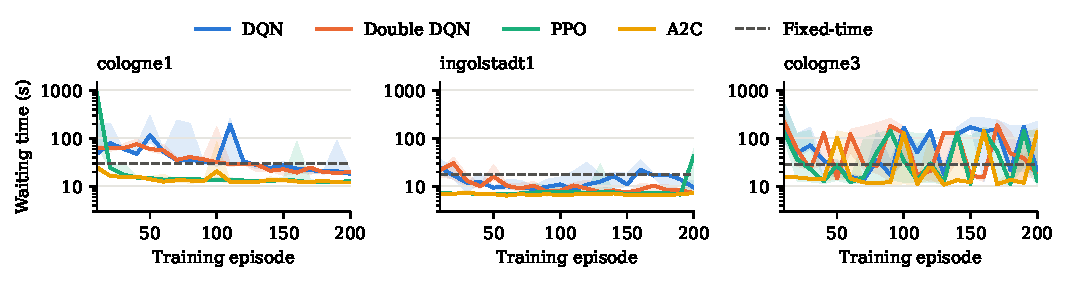
\includegraphics[width=\textwidth]{figures/learning_curves.pdf}
  \caption{Validation waiting time during training.}
  \label{fig:curves}
\end{figure*}

\subsection{Training Stability and Failure Analysis}
Fig.~\ref{fig:curves} shows the complete learning curves, the validation waiting time at every check, on a logarithmic scale so that gridlocked checkpoints remain visible; each line is the median over the five seeds, the band the interquartile range across seeds, and the dashed line fixed-time control. On cologne1 the median A2C and PPO policies beat fixed-time from episodes 10 and 20, and DQN and Double DQN only from 130 and 110; on ingolstadt1 all learners do so within 30 episodes. On cologne3 the validation score oscillates between good and gridlocked policies throughout training: after episode 50, 32\% (A2C), 41\% (PPO, Double DQN) and 48\% (DQN) of the checks are over twice as bad as fixed-time, against 0--11\% on ingolstadt1 and 7--23\% on cologne1.

Failures are rare but severe: a failed episode completes only 31--92\% of trips, against 98.8\% otherwise, which is why mean and median diverge. On cologne3 the median per-seed waiting times of A2C, PPO and Double DQN (13.8, 14.1 and 15.2\,s) are 51--55\% below fixed-time. Selecting the checkpoint on five validation files does not prevent rare failures, since even A2C failed on one of 50 cologne3 test episodes. A likely cause is spillback between adjacent intersections, invisible to the local reward of Section~\ref{sec:problem}.

\subsection{Ablation Study}
\label{sec:ablation}
Table~\ref{tab:ablation} removes one framework component at a time from A2C, the best learner, holding the seeds, hyperparameters, interaction budget and test conditions fixed.

Removing demand-randomized training (C1), i.e.\ training only on the real hour, gives a slightly lower waiting time on that same hour on cologne1 (11.0 vs.\ 11.7\,s), a sign of fitting the training demand; one cologne1 seed then gridlocks at $1.3\times$, and on cologne3 failures rise from 1 to 6 of 50 test episodes (Mann--Whitney $U$ on all test files, $p=0.032$; cologne1 $p=0.42$). Removing policy sharing (C2), i.e.\ one network per cologne3 signal with 34{,}373 instead of 11{,}845 parameters and 3.4 instead of 4.0 CPU-hours of training, gives 4 failures ($p=0.056$). Episodes without gridlock are, however, almost identical in all variants ($1.0\times$: 10.0--10.7\,s), so neither component changes typical performance.

Valid-action masking differs from the full framework only in how the surplus action of the three-phase signal is handled. It also leaves typical performance unchanged and is the most consistent variant on unseen demand (16.8\,$\pm$\,0.7\,s), but it fails in 4 of 50 episodes and in four of five seeds, as often as the ablated variants, and is worse than the unmasked policy over all test files ($p=0.032$). Since a near-identical configuration fails as often as the ablated ones, the low failure count of the full framework is likely due in part to its five seeds, and with five seeds the effect of C1 and C2 on failures is indicative rather than established. Table~\ref{tab:perint} locates the failures: in every variant A2C cuts the mean queue at signals A and B from about 3 vehicles under fixed-time to 0.5--1.7, whereas at signal C, the largest junction, the variants with failing seeds queue almost as much as fixed-time (5.3--6.1 vs.\ 6.8 vehicles).

\begin{table}[t]
\caption{Ablation of A2C (Waiting Time in s)}
\label{tab:ablation}
\centering
\footnotesize
\setlength{\tabcolsep}{2pt}
\resizebox{\columnwidth}{!}{%
\begin{tabular}{|l|l|r|r|r|r|}
\hline
\textbf{Scen.} & \textbf{Variant} & \textbf{Unseen\textsuperscript{a}} & \textbf{Real hour} & \textbf{F} & \textbf{Params} \\
\hline
\multirow{2}{*}{cologne1} & Full (C1 + C2)          & 15.6\,$\pm$\,1.0  & 11.7\,$\pm$\,0.7    & 0 & 11{,}461 \\ \cline{2-6}
                          & $-$C1 (real hour only)  & 25.5\,$\pm$\,25.4 & 11.0\,$\pm$\,0.3    & 1 & 11{,}461 \\
\hline
\multirow{4}{*}{cologne3} & Full (C1 + C2)          & 36.0\,$\pm$\,45.3 & 9.3\,$\pm$\,0.6     & 1 & 11{,}845 \\ \cline{2-6}
                          & $-$C1 (real hour only)  & 66.1\,$\pm$\,66.3 & 122.7\,$\pm$\,227.1 & 6 & 11{,}845 \\ \cline{2-6}
                          & $-$C2 (one per signal)  & 94.6\,$\pm$\,78.4 & 157.1\,$\pm$\,329.8 & 4 & 34{,}373 \\ \cline{2-6}
                          & Full + masking          & 16.8\,$\pm$\,0.7  & 133.6\,$\pm$\,277.1 & 4 & 11{,}845 \\
\hline
\end{tabular}}
\tablenote{Mean $\pm$ s.d.\ over 5 seeds. \textsuperscript{a}The $0.7\times$ and $1.3\times$ test files. F: failed test episodes out of 50. Params: actor and critic.}
\end{table}

\begin{table}[t]
\caption{Mean Queue per Signal on cologne3}
\label{tab:perint}
\centering
\footnotesize
\setlength{\tabcolsep}{4pt}
\begin{tabular}{|l|c|c|c|}
\hline
\textbf{Controller} & \textbf{\makecell{Signal A\\(3 phases)}} & \textbf{\makecell{Signal B\\(4 phases)}} & \textbf{\makecell{Signal C\\(4 phases)}} \\
\hline
Fixed-time          & 3.08 & 3.03 & 6.77 \\
\hline
A2C, shared         & 0.51\,$\pm$\,0.07 & 0.54\,$\pm$\,0.40 & 2.65\,$\pm$\,2.16 \\
\hline
A2C, one per signal & 0.59\,$\pm$\,0.19 & 1.65\,$\pm$\,1.28 & 6.13\,$\pm$\,2.41 \\
\hline
A2C, shared, masked & 0.54\,$\pm$\,0.02 & 0.89\,$\pm$\,0.48 & 5.33\,$\pm$\,2.32 \\
\hline
\end{tabular}
\tablenote{Halted vehicles on each signal's incoming lanes, averaged over the hour and the ten test files; mean $\pm$ s.d.\ over 5 seeds.}
\end{table}

Several challenges remain and set the directions for future work. The most pressing is the rare gridlock of multi-intersection policies, concentrated at the largest junction, which neither validation-based selection, the framework components nor action masking reliably remove; the local, myopic reward is a likely cause, and coordination-aware rewards, a safe fallback to fixed-time control and more training seeds are natural next steps. The test covers demand-level generalization only, the shared policy is tied to the training intersections through its identifier, and the results are simulation-only, so the sim-to-real gap~\cite{rafi2026sim2signal} remains open. Future work will also compress the best learner for roadside devices, building on compact controllers~\cite{xing2022tinylight,gu2024pilight}, and add multi-tier anomaly detection and confidence-aware edge--cloud offloading.

\section{Conclusion}
\label{sec:conclusion}

This paper compared DQN, Double DQN, PPO and A2C for traffic signal control on three real-city RESCO scenarios, using a generalization-focused framework of demand-randomized training and a shared policy, and testing only on demand unseen in training. A2C was the best and most robust learner, reducing waiting time by 58--59\% on the single-intersection scenarios and keeping more than half of that advantage at unseen heavy demand. On the three-intersection corridor every learner occasionally gridlocked the network at its largest junction, and neither demand randomization, policy sharing nor action masking reliably prevented it. Reliable multi-intersection control, rather than average performance, is therefore the main obstacle to deploying these controllers.


% References: kept in the separate file references.bib
\balance
\bibliographystyle{IEEEtran}
\bibliography{references}

\end{document}
